% ----------------------------------------------------------
% Desenvolvimento do Projeto
% ----------------------------------------------------------
\chapter{Desenvolvimento do Projeto}
\label{cha:desenvolvimento}

Este capítulo detalha as etapas de concepção, modelagem e implementação do sistema \textit{SyncCarreira}. O foco estrutural deste documento abrange desde o levantamento inicial de requisitos até a definição da arquitetura de \textit{back-end} e das estratégias de segurança e implantação, garantindo a robustez necessária para o processamento de dados sensíveis no contexto de testes vocacionais.

\section{Escopo do Projeto}

O escopo deste projeto compreende o desenvolvimento de uma plataforma \textit{Web} responsiva, estruturada no modelo \textit{Software as a Service} (SaaS), voltada para a automação e gestão de testes vocacionais em instituições de ensino. O sistema visa atender a três perfis distintos de usuários: Administrador, Psicóloga Escolar e Aluno.

Para solucionar o problema de lentidão e processos manuais na orientação vocacional, o sistema entregará as seguintes funcionalidades:

\begin{itemize}
    \item \textbf{Módulo de Autenticação e Autorização:} Sistema de \textit{login} seguro com controle de acesso baseado em perfis (\textit{Role-Based Access Control}), garantindo o isolamento de dados entre diferentes instituições e usuários.

    \item \textbf{Gestão Dinâmica de Testes:} Ferramenta administrativa que permite às psicólogas cadastrar, editar, visualizar e excluir testes vocacionais, inserindo perguntas, escalas e pesos personalizados diretamente na plataforma.

    \item \textbf{Módulo do Aluno:} Interface interativa e gamificada (utilizando componentes como a Escala Likert) para a realização dos testes vocacionais de forma digital.

    \item \textbf{Feedback Instantâneo:} O motor do sistema processará as respostas em tempo real e, ao finalizar a submissão, fornecerá um \textit{feedback} imediato na tela do aluno com o seu perfil vocacional calculado.

    \item \textbf{Motor de Avaliação (\textit{Back-end}):} Algoritmo responsável por receber as respostas do aluno, tabular os dados com base nos pesos pré-definidos e calcular o perfil vocacional resultante.

    \item \textbf{Módulo da Psicóloga (\textit{Dashboard}):} Painel de gestão em que a profissional poderá visualizar a lista de alunos de sua instituição, acompanhar o \textit{status} de preenchimento dos testes e acessar os relatórios finais com os resultados consolidados de cada estudante.

    \item \textbf{Painel da Psicóloga (Filtros e Classificação):} Painel de gestão em que o profissional poderá acompanhar o progresso dos testes. O módulo contará com ferramentas de filtragem avançada, permitindo classificar e agrupar os alunos por turma e por resultado vocacional.

    \item \textbf{Agendamento de Consultas:} Módulo integrado de calendário que permite à psicóloga marcar, organizar e gerenciar horários de atendimento e sessões de orientação individual com os alunos a partir do sistema.

    \item \textbf{Módulo Administrativo:} Funcionalidades para o cadastro de escolas, psicólogas e alunos na base de dados.
\end{itemize}

\subsection{Regras de negócio}

As regras de negócio estabelecem as políticas, as restrições e as diretrizes operacionais que o software SyncCarreira deve seguir para garantir a eficácia do seu propósito pedagógico e terapêutico. Segundo a literatura de Engenharia de Software, a definição clara dessas regras é o que garante que o sistema reflita adequadamente as necessidades, os processos e os limites do domínio do problema, servindo como base para a validação dos requisitos \cite{sommerville2011, pressman2016}.

A dinâmica principal do sistema fundamenta-se em uma progressão estruturada, na qual a jornada do aluno é dividida em quatro trilhas sequenciais obrigatórias: autoconhecimento, influências, informação e projeto de futuro. Como mecanismo de controle de fluxo, o avanço na plataforma é estritamente condicionado à conclusão da etapa anterior. Durante esse processo, o sistema assegura a autonomia do estudante, permitindo que ele expresse suas opiniões e sentimentos livremente, culminando na elaboração de uma síntese textual ao final de cada trilha.

Em alinhamento com as diretrizes contemporâneas de orientação profissional, que compreendem a escolha de carreira como um processo construído socialmente em vez da revelação de uma vocação inata (BOCK, 2004), o software atua estritamente como uma ferramenta facilitadora. O sistema não valida nem fornece conteúdo psicológico proprietário; a curadoria e a formulação das perguntas são de inteira responsabilidade da instituição e do profissional de psicologia. Consequentemente, o resultado final entregue pelo sistema não consiste em um diagnóstico fechado de carreira, mas sim na apresentação de um leque amplo de possibilidades, garantindo que o aluno possua um panorama completo do seu processo de escolha. No pilar de Informação, a plataforma deve assegurar que o aluno acesse links previamente curados pela psicóloga, direcionando-o a fontes externas seguras e confiáveis, como portais do Enem, ProUni, políticas de cotas e informações sobre cursos.

Por fim, os mecanismos de monitoramento foram projetados para otimizar o tempo e a intervenção da psicóloga escolar, garantindo que ela consiga dar atenção especial àqueles alunos que apresentam dificuldades. Para respeitar as normas de atuação profissional e manter o foco na gestão das turmas, o painel da psicóloga exibirá um indicador de status de conclusão por aluno e acionará um alerta visual (flag) de "necessidade de orientação", preservando, nesse nível gerencial, o sigilo sobre o detalhe de cada resposta fornecida. O sistema também incorpora regras de triagem terapêutica, nas quais os alunos que já possuem todas as trilhas concluídas, mas permanecem com o status "em dúvida", são imediatamente priorizados para a participação em sessões de orientação em grupo.

Para uma visualização objetiva e rastreabilidade durante o desenvolvimento, a Tabela 1 descreve as regras de negócio mapeadas para a plataforma.

\begin{table}[htb]
    \centering
    \ABNTEXfontereduzida
    \caption[Regras de Negócio do SyncCarreira]{Regras de negócio do SyncCarreira.}
    \label{tab-regras-negocio}
    \begin{tabular}{|c|p{12cm}|}
    \hline
    \textbf{Identificador} & \multicolumn{1}{c|}{\textbf{Regra de Negócio}} \\
    \hline
    \textbf{RN-01} & A jornada do aluno é dividida em 4 trilhas sequenciais (autoconhecimento, influências, informação, projeto de futuro). Não é possível avançar sem concluir a trilha anterior. \\
    \hline
    \textbf{RN-02} & O aluno precisa ter autonomia para realizar as trilhas e expressar sua opinião/sentimentos. Ao final de cada trilha, o aluno deve obrigatoriamente registrar uma síntese textual livre. \\
    \hline
    \textbf{RN-03} & O painel da psicóloga deve exibir o status por aluno (trilhas concluídas) e acionar uma \textit{flag} de "necessidade de orientação" para alunos com dificuldades, sem exibir, neste painel, os detalhes das respostas individuais. \\
    \hline
    \textbf{RN-04} & Alunos que concluíram todas as trilhas, mas permanecem com o status "em dúvida", devem ser priorizados automaticamente pelo sistema para sessões de orientação em grupo. \\
    \hline
    \textbf{RN-05} & No pilar de Informação, o sistema deve fornecer aos alunos links previamente curados pela psicóloga direcionados a fontes externas confiáveis (Enem, ProUni, cotas, cursos disponíveis). \\
    \hline
    \textbf{RN-06} & O sistema não valida nem fornece conteúdo psicológico proprietário. A instituição/psicóloga é inteiramente responsável por criar e inserir as perguntas (trilhas) dentro da ferramenta. \\
    \hline
    \textbf{RN-07} & O resultado final gerado pela jornada deve apresentar um leque de possibilidades formativas e profissionais, sendo proibida a geração de um diagnóstico fechado de carreira. \\
    \hline
    \textbf{RN-08} & O sistema deve fornecer ao aluno um panorama completo do seu histórico na jornada, garantindo uma visão holística e contínua do seu processo de escolha. \\
    \hline
    \end{tabular}
    \legend{Fonte: Autoria própria (2026).}
    \end{table}

\subsection{Requisitos Funcionais}

Os requisitos funcionais descrevem as ações e os comportamentos específicos que o software SyncCarreira deve executar para atender às necessidades dos seus diferentes perfis de usuários. Eles definem "o que" o sistema fará, delineando as interações fundamentais entre os atores e a plataforma.

A arquitetura de funcionalidades do sistema foi distribuída entre três atores principais: o Administrador, a Psicóloga e o Aluno. O administrador detém permissões de alto nível para cadastrar, editar e desativar instituições (escolas ou ONGs) na plataforma, além de criar e gerenciar as contas de usuários com permissões isoladas por perfil. A psicóloga, atuando como curadora pedagógica, possui acesso para criar e organizar perguntas customizadas nas quatro trilhas fundamentais. Além disso, o sistema fornece à profissional um painel de monitoramento que exibe o status de cada aluno e gera alertas automáticos (flags) para aqueles que concluíram as trilhas mas indicaram indecisão, priorizando-os para agendamentos de sessões e permitindo a emissão de relatórios individuais ou de turma. A psicóloga também conta com ferramentas para enviar feedbacks personalizados e curar links de fontes externas.

Do lado do aluno, o sistema exige a navegação obrigatória pelas quatro trilhas sequenciais (autoconhecimento, influências, informação e projeto de futuro). A plataforma garante a autonomia do estudante, permitindo o registro de sínteses textuais ao final de cada etapa e a livre expressão por meio de campos abertos e escalas. Como entrega de valor, o sistema fornece ao estudante a visualização de um leque de possibilidades de carreira ao final da jornada, o acompanhamento do seu histórico de testes, a personalização de interesses e o acesso direto aos seus agendamentos e feedbacks enviados pela profissional.

A Tabela 2 detalha todos os requisitos funcionais mapeados para o MVP do SyncCarreira e suas respectivas prioridades. 

\begin{table}[H]
    \centering
    \ABNTEXfontereduzida
    \caption[Requisitos Funcionais do SyncCarreira]{Requisitos funcionais do SyncCarreira.}
    \label{tab-requisitos-funcionais}
    \begin{tabular}{|c|p{3cm}|p{5.5cm}|c|c|c|}
    \hline
    \rowcolor{blue!80!black}
    \textcolor{white}{\textbf{ID}} & 
    \textcolor{white}{\textbf{Título}} & 
    \textcolor{white}{\textbf{Descrição}} & 
    \textcolor{white}{\textbf{Regras}} & 
    \textcolor{white}{\textbf{Ator}} & 
    \textcolor{white}{\textbf{Prior.}} \\
    \hline
    
    \textcolor{blue!70!black}{\textbf{RF-01}} & 
    \textbf{Cadastro de instituições} & 
    O administrador deve poder cadastrar, editar e desativar instituições (escolas/ONGs) na plataforma, associando a cada uma seus usuários e turmas. & 
    --- & 
    Administrador & 
    \textcolor{red!80!black}{\textbf{Alta}} \\
    \hline
    
    \textcolor{blue!70!black}{\textbf{RF-02}} & 
    \textbf{Gestão de usuários e perfis de acesso} & 
    O administrador deve poder criar, editar e desativar contas de psicólogas e alunos, atribuindo o perfil correto (administrador, psicóloga, aluno) com permissões isoladas por perfil. & 
    --- & 
    Administrador & 
    \textcolor{red!80!black}{\textbf{Alta}} \\
    \hline
    
    \textcolor{blue!70!black}{\textbf{RF-03}} & 
    \textbf{Criação e gestão de perguntas e trilhas} & 
    A psicóloga deve poder criar, editar e excluir perguntas e organizá-las em trilhas customizadas, associadas aos quatro pilares (autoconhecimento, influências, informação, projeto de futuro). O conteúdo é de responsabilidade da instituição. & 
    RN-06 & 
    Psicóloga & 
    \textcolor{red!80!black}{\textbf{Alta}} \\
    \hline
    
    \textcolor{blue!70!black}{\textbf{RF-04}} & 
    \textbf{Painel de monitoramento de status por aluno} & 
    A psicóloga deve visualizar, em um painel, o status de progresso de cada aluno por trilha concluída, sem necessidade de ler resposta por resposta. & 
    RN-03 & 
    Psicóloga & 
    \textcolor{red!80!black}{\textbf{Alta}} \\
    \hline
    
    \textcolor{blue!70!black}{\textbf{RF-05}} & 
    \textbf{Flag de necessidade de orientação} & 
    O sistema deve sinalizar automaticamente alunos que concluíram todas as trilhas mas \textit{permanecem com o status "em dúvida"}. & 
    RN-03, RN-04 & 
    Psicóloga & 
    \textcolor{red!80!black}{\textbf{Alta}} \\
    \hline
    
    \end{tabular}
    \legend{Fonte: Autoria própria (2026).}
\end{table}

\subsection{Requisitos Funcionais}

Enquanto os requisitos funcionais definem o que o sistema fará, os requisitos não funcionais especificam "como" ele deve operar, estabelecendo os atributos de qualidade, as restrições tecnológicas e as exigências de desempenho e segurança da aplicação.

Para o SyncCarreira, a proteção da informação é um pilar crítico, dado o tratamento de dados de menores de idade. Nesse sentido, o sistema implementará controle de autenticação utilizando tokens JWT para impedir acessos cruzados entre perfis e adotará criptografia em repouso para os dados sensíveis, garantindo estrita conformidade com a Lei Geral de Proteção de Dados (LGPD) e permitindo a exclusão de registros a pedido da instituição. A arquitetura SaaS impõe também que haja um isolamento lógico completo dos dados, impedindo que informações de alunos e turmas sejam acessadas por outras instituições cadastradas.

No aspecto de usabilidade e performance, o software requer uma interface responsiva (focada em mobile-first), acessível e intuitiva para o público jovem. As operações fundamentais devem manter um tempo de resposta inferior a 2 segundos e a disponibilidade do sistema deve ser garantida em 99% durante o período letivo comercial. A sustentabilidade técnica do back-end será viabilizada pela utilização de uma arquitetura em camadas em Java com Spring Boot, aliada à documentação automática da API via Swagger/OpenAPI, assegurando manutenibilidade e escalabilidade para versões futuras.

A Tabela 6 sistematiza as premissas não funcionais adotadas para o projeto.

\begin{table}[H]
    \centering
    \ABNTEXfontereduzida
    \caption[Requisitos Não Funcionais do SyncCarreira]{Requisitos não funcionais do SyncCarreira.}
    \label{tab-requisitos-nao-funcionais}
    \begin{tabular}{|c|p{3.5cm}|p{5cm}|c|c|c|}
    \hline
    \rowcolor{blue!80!black}
    \textcolor{white}{\textbf{ID}} & 
    \textcolor{white}{\textbf{Título}} & 
    \textcolor{white}{\textbf{Descrição}} & 
    \textcolor{white}{\textbf{Regras}} & 
    \textcolor{white}{\textbf{Ator}} & 
    \textcolor{white}{\textbf{Prior.}} \\
    \hline
    
    \textcolor{blue!70!black}{\textbf{RNF-01}} & 
    \textbf{Segurança — autenticação e autorização} & 
    O sistema deve implementar autenticação via token JWT com expiração configurável. O acesso a cada recurso deve ser validado pelo perfil do usuário (administrador, psicóloga, aluno), impedindo acesso cruzado entre perfis. & 
    --- & 
    Sistema & 
    \textcolor{red!80!black}{\textbf{Alta}} \\
    \hline
    
    \textcolor{blue!70!black}{\textbf{RNF-02}} & 
    \textbf{Privacidade e proteção de dados (LGPD)} & 
    Dados sensíveis de menores de idade (sínteses, respostas, perfil) devem ser armazenados com criptografia em repouso. O sistema deve permitir exclusão de dados a pedido da instituição, em conformidade com a LGPD. & 
    --- & 
    Sistema & 
    \textcolor{red!80!black}{\textbf{Alta}} \\
    \hline
    
    \textcolor{blue!70!black}{\textbf{RNF-03}} & 
    \textbf{Desempenho — tempo de resposta} & 
    As operações principais (carregamento de trilha, salvamento de resposta, exibição do painel) devem responder em até 2 segundos em condições normais de uso. & 
    --- & 
    Sistema & 
    \textcolor{orange!90!black}{\textbf{Média}} \\
    \hline
    
    \textcolor{blue!70!black}{\textbf{RNF-04}} & 
    \textbf{Usabilidade — interface acessível e responsiva} & 
    A interface deve ser responsiva (mobile-first), legível e navegável por jovens sem familiaridade técnica. A jornada do aluno deve ser intuitiva, sem necessidade de manual. & 
    --- & 
    Sistema & 
    \textcolor{red!80!black}{\textbf{Alta}} \\
    \hline
    
    \textcolor{blue!70!black}{\textbf{RNF-05}} & 
    \textbf{Disponibilidade} & 
    O sistema deve ter disponibilidade mínima de 99\% durante o horário comercial. & 
    --- & 
    Sistema & 
    \textcolor{orange!90!black}{\textbf{Média}} \\
    \hline
    
    \end{tabular}
    \legend{Fonte: Autoria própria (2026).}
    \end{table}

\section{Histórias de Usuário}

O projeto \textit{SyncCarreira} adota a metodologia ágil Scrum, utilizando Histórias de Usuário (HU) para orientar o desenvolvimento de todo o ecossistema da plataforma, desde a jornada básica do MVP até as funcionalidades de gestão avançada previstas para a conclusão do projeto. As histórias a seguir refletem as necessidades de todos os perfis de usuários identificados.

\subsection{Descrição das Histórias de Usuário}

\paragraph{Perfil: Psicólogo (Gestão, Intervenção e Acompanhamento)}

\begin{itemize}
    \item \textbf{HU01 -- Monitoramento de Turma:} Como psicólogo, quero um painel de monitoramento de \textit{status} por turma, para que eu visualize o progresso dos alunos sem acessar dados sigilosos. \\
    \textit{Critérios de Aceitação:} O sistema deve exibir lista de alunos por turma; filtrar por trilhas concluídas.

    \item \textbf{HU02 -- Triagem de Necessidades:} Como psicólogo, quero visualizar alunos com dificuldades ou indecisos, para priorizar sessões (RN-03, RN-04). \\
    \textit{Critérios de Aceitação:} Sistema deve gerar alerta visual (\textit{flag}) para alunos com \textit{status} "em dúvida".

    \item \textbf{HU03 -- Customização de Trilhas:} Como psicólogo, quero criar e organizar trilhas customizadas, adaptando o conteúdo à necessidade da turma (RN-06). \\
    \textit{Critérios de Aceitação:} Permitir cadastro, edição e exclusão de perguntas e trilhas.

    \item \textbf{HU04 -- Curadoria de Materiais:} Como psicólogo, quero realizar a curadoria de \textit{links} externos, oferecendo material de consulta confiável (RN-05). \\
    \textit{Critérios de Aceitação:} Permitir associar \textit{links} de fontes externas à trilha de "Informação".

    \item \textbf{HU05 -- Emissão de Relatórios:} Como psicólogo, quero gerar relatórios de turma e individuais, para embasar \textit{feedbacks} técnicos. \\
    \textit{Critérios de Aceitação:} Exportar panorama macro da turma e histórico detalhado do aluno.

    \item \textbf{HU06 -- Comunicação de Feedback:} Como psicólogo, quero enviar \textit{feedbacks} personalizados pela plataforma, centralizando a análise e orientações. \\
    \textit{Critérios de Aceitação:} Disponibilizar campo de texto editável para \textit{feedback} enviado ao aluno.

    \item \textbf{HU07 -- Gestão de Agendamentos:} Como psicólogo, quero gerenciar o agendamento de sessões (individuais ou grupo), visualizando-as por calendário. \\
    \textit{Critérios de Aceitação:} Notificar aluno automaticamente sobre o agendamento criado.
\end{itemize}

\paragraph{Perfil: Aluno (Engajamento, Reflexão e Organização)}

\begin{itemize}
    \item \textbf{HU08 -- Jornada de Aprendizado:} Como aluno, quero percorrer trilhas sequenciais, absorvendo conteúdo de forma lógica e gradativa (RN-01). \\
    \textit{Critérios de Aceitação:} Bloquear acesso à trilha seguinte enquanto a atual não for concluída.

    \item \textbf{HU09 -- Registro de Síntese:} Como aluno, quero registrar sínteses textuais ao final de cada trilha, expressando minhas reflexões (RN-02). \\
    \textit{Critérios de Aceitação:} Campo de texto obrigatório para finalização de cada trilha.

    \item \textbf{HU10 -- Panorama e Resultados:} Como aluno, quero visualizar leque de carreiras e histórico de trilhas, compreendendo minha evolução (RN-07, RN-08). \\
    \textit{Critérios de Aceitação:} Exibir áreas sugeridas sem emitir diagnóstico fechado.

    \item \textbf{HU11 -- Organização de Agenda:} Como aluno, quero visualizar meus agendamentos e \textit{feedbacks} recebidos, acompanhando meu progresso. \\
    \textit{Critérios de Aceitação:} Exibir área dedicada no painel do aluno com o histórico de sessões.

    \item \textbf{HU12 -- Configuração de Perfil:} Como aluno, quero personalizar meu perfil e selecionar interesses, tornando a experiência mais alinhada às minhas afinidades. \\
    \textit{Critérios de Aceitação:} Permitir que o aluno atualize seus interesses declarados.
\end{itemize}

\paragraph{Perfil: Administrador (Governança, Segurança e Escala)}

\begin{itemize}
    \item \textbf{HU13 -- Cadastro e Gestão de Instituições:} Como administrador, quero cadastrar e gerir múltiplas instituições (escolas/ONGs), para que eu possa escalar o uso da plataforma para diferentes parceiros de forma isolada (RF-01). \\
    \textit{Critérios de Aceitação:} O sistema deve permitir o cadastro de nome, CNPJ e configurações de acesso da instituição; os dados devem ser logicamente segregados por ID de instituição.

    \item \textbf{HU14 -- Gestão de Perfis e Isolamento de Acesso:} Como administrador, quero gerir contas de psicólogas e alunos, atribuindo permissões específicas, para garantir que usuários acessem apenas os dados de sua própria instituição (RF-02, RNF-08). \\
    \textit{Critérios de Aceitação:} O sistema deve validar o perfil (Admin, Psicólogo, Aluno) em cada requisição; deve impedir o acesso cruzado de dados entre instituições.

    \item \textbf{HU15 -- Auditoria e Conformidade LGPD:} Como administrador, quero ferramentas para exclusão de dados e gestão de termos de uso, para que a plataforma permaneça em conformidade com a LGPD (RNF-02). \\
    \textit{Critérios de Aceitação:} Deve haver uma funcionalidade para a exclusão irreversível de dados de alunos a pedido da instituição ou responsável legal.
\end{itemize}

\section{Arquitetura}

O software \textit{SyncCarreira}. adota o modelo de implantação \textit{Software as a Service} (SaaS), focado na distribuição do sistema em nuvem para instituições de ensino. Sob a ótica do desenvolvimento web, o projeto foi concebido a partir da separação das responsabilidades entre o cliente e o servidor, sendo a comunicação intermediada por uma API REST.

Para a camada de visualização, o sistema utiliza a abordagem de \textit{Single Page Application} (SPA), a qual propicia uma experiência de uso responsiva, interativa e econômica no consumo de banda, visto que dispensa recarregamentos completos de página a cada interação do usuário. No que tange à lógica do servidor, a aplicação fundamenta-se no padrão de Arquitetura em Camadas (Layered Architecture). Esse padrão, amplamente consolidado no ecossistema Spring Boot, assegura que o código seja altamente coeso e de baixo acoplamento, já que cada camada detém uma finalidade delimitada e apenas se comunica de modo estrito com as camadas diretamente adjacentes.


\subsection{Definições da Arquitetura}

O \textit{SyncCarreira} foi estruturado com base em uma Arquitetura em Camadas (\textit{Layered Architecture}), que garante a separação de responsabilidades entre a interface de usuário, a lógica de negócios e a persistência de dados. Esta definição arquitetural prioriza a manutenibilidade, permitindo que alterações na interface ou nas regras de negócio ocorram sem impactar o núcleo do sistema.

O sistema gerencia o ciclo de vida da informação através de módulos de alta coesão, abstraindo operações básicas de persistência para níveis de governança e orquestração de dados:

\subsection{Diagrama da Arquitetura}

O diagrama abaixo ilustra a arquitetura técnica do sistema, detalhando a infraestrutura em nuvem e a integração entre os componentes da aplicação:

\begin{figure}[htb]
    \centering
    \caption{Representação da Arquitetura de Infraestrutura e Implantação (AWS Cloud).}
    \label{fig_arquitetura}
    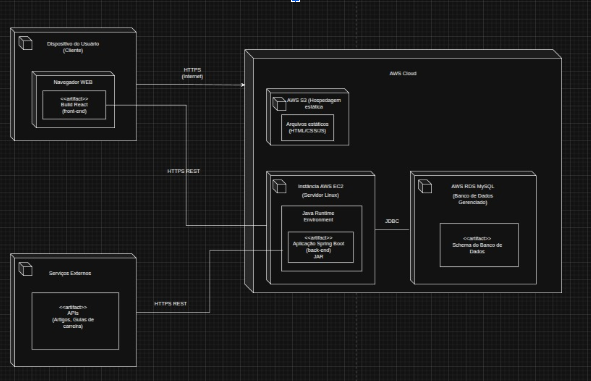
\includegraphics[width=0.90\textwidth]{img/diag-1-arquitetura-infraestrutura-aws.png}
    \legend{Fonte: Produzido pelos autores (2026).}
\end{figure}


A arquitetura foi estruturada para garantir escalabilidade e segurança, composta pelos seguintes elementos principais:

\begin{itemize}
    \item \textbf{Dispositivo do Usuário:} Interface \textit{front-end} desenvolvida em React, acessada via navegador \textit{web} e comunicando-se via HTTPS com os serviços em nuvem.

    \item \textbf{AWS S3:} Responsável pela hospedagem dos arquivos estáticos (HTML/CSS/JS), garantindo alta disponibilidade e \textit{performance} no carregamento da interface.

    \item \textbf{Instância AWS EC2:} Servidor Linux que hospeda o \textit{back-end} desenvolvido em Java/\textit{Spring Boot}, processando as regras de negócio e gerenciando as requisições REST.

    \item \textbf{AWS RDS (MySQL):} Banco de dados gerenciado que garante a persistência das entidades do sistema, com conexão segura via JDBC realizada diretamente pelo \textit{back-end}.
\end{itemize}

\section{Tecnologias}

O ecossistema tecnológico do \textit{SyncCarreira} foi selecionado para garantir robustez, segurança e escalabilidade, permitindo que a aplicação suporte desde a operação do MVP até a consolidação do projeto completo. Abaixo, detalham-se as tecnologias adotadas para cada componente da solução.

\subsection{Front-end}

O \textit{front-end} foi desenvolvido com abordagem \textit{mobile-first}, utilizando HTML, CSS e JavaScript para garantir uma interface intuitiva e acessível. A biblioteca React foi aplicada na estruturação de componentes reutilizáveis, otimizando a navegação, garantindo fluidez e assegurando uma experiência dinâmica e adaptável aos diversos dispositivos dos estudantes.

\subsection{Back-end}

O \textit{back-end} utiliza Java com o \textit{framework} \textit{Spring Boot}, estruturado sob o padrão de arquitetura em camadas (Controller, Service, Repository, Entity), o que garante a separação de responsabilidades, facilidade de manutenção e a robustez necessária para as regras de negócio complexas das trilhas vocacionais.

\subsection{Banco de Dados}

O sistema utiliza o banco de dados MySQL para o armazenamento das entidades e registros da plataforma, garantindo a integridade, a consistência dos dados e o suporte eficiente às transações relacionais necessárias para o funcionamento das trilhas de orientação e perfis de usuário.

\subsection{Infraestrutura}

A estratégia de infraestrutura baseia-se em um modelo SaaS (\textit{Software as a Service}) hospedado na nuvem, garantindo alta disponibilidade para os usuários finais.

\subsubsection{Amazon Web Services (AWS)}

A aplicação é hospedada na AWS (\textit{Amazon Web Services}), aproveitando a infraestrutura global para garantir a disponibilidade exigida para o horário letivo. Além disso, a segurança baseada em \textit{tokens} JWT (\textit{JSON Web Token}) é implementada para garantir a autorização e o isolamento lógico entre os diferentes perfis (Administrador, Psicóloga e Aluno) e entre diferentes instituições, cumprindo as diretrizes de segurança da informação.

\section{Testes e Manutenibilidade}

A estratégia de testes do \textit{SyncCarreira} foi concebida para assegurar a confiabilidade, a segurança dos dados e a conformidade com as regras de negócio estabelecidas, garantindo que o sistema evolua de forma estável durante todo o ciclo de desenvolvimento.

\subsection{Plano de Testes}

O plano de testes adota uma abordagem em camadas, onde a qualidade é validada desde o desenvolvimento unitário até a aceitação final. A estratégia foca na automação de processos, visando reduzir falhas em produção e garantir a integridade do isolamento de dados entre diferentes instituições. Os testes são executados automaticamente através do Maven em cada ciclo de \textit{build}, assegurando que novas implementações não comprometam funcionalidades existentes.

A execução do plano de testes contempla:

\begin{itemize}
    \item \textbf{Testes Funcionais e Unitários:} Validação da lógica de negócio e componentes isolados via JUnit, garantindo que as regras de cada trilha operem conforme o esperado.

    \item \textbf{Testes de Integração:} Validação da persistência de dados utilizando o banco H2, confirmando a comunicação correta entre as camadas Repository e o banco.

    \item \textbf{Testes Não Funcionais:} Avaliação de \textit{performance} e carga, monitorando o tempo de resposta das consultas principais (meta de até 2s) e a disponibilidade do sistema em períodos de alta demanda escolar.

    \item \textbf{Análise Estática e Convenções:} Aplicação de padrões de \textit{clean code} e documentação de API via Swagger, facilitando a manutenibilidade do código por terceiros.
\end{itemize}

\section{Segurança, Privacidade e Legislação}

Esta seção estabelece os compromissos do \textit{SyncCarreira} com a proteção de dados e a conformidade legal, priorizando um ambiente de confiança para a interação entre alunos, psicólogos e instituições de ensino. A segurança da informação é tratada como um requisito fundamental para a operação do sistema, assegurando que o tratamento de dados pessoais ocorra de forma ética e protegida.

\subsection{Critérios de Segurança e Privacidade}

O sistema foi projetado para garantir que as informações de cada participante permaneçam restritas ao contexto da sua própria instituição de ensino. O acesso à plataforma é rigorosamente controlado, assegurando que cada usuário --- seja ele aluno, psicólogo ou administrador --- visualize apenas os dados necessários para o exercício de sua função. Essa estrutura de governança impede o cruzamento de informações entre diferentes escolas ou grupos, protegendo o sigilo e a privacidade dos registros individuais. Além disso, todas as informações sensíveis dos estudantes são armazenadas com proteção rigorosa contra acessos não autorizados, reforçando o cuidado necessário com a jornada de autodescoberta dos jovens.

\subsection{Observância à Legislação}

O \textit{SyncCarreira} está em conformidade com as diretrizes da Lei Geral de Proteção de Dados (LGPD), tratando a privacidade como um compromisso central do serviço prestado. A plataforma foi estruturada para respeitar o direito de controle do usuário sobre seus próprios dados, oferecendo mecanismos que permitem às instituições parceiras gerenciar a permanência das informações, incluindo o procedimento para exclusão ou anonimização dos registros quando o vínculo do aluno com a escola é finalizado. O sistema assegura que os dados coletados sejam utilizados exclusivamente para a finalidade de orientação vocacional, garantindo total transparência e conformidade com o cenário legal vigente para o tratamento de dados pessoais no ambiente educacional.

\section{Modelo de Banco de Dados}

Este tópico apresenta a estrutura de dados do \textit{SyncCarreira}, projetada para organizar as informações dos usuários, o fluxo das trilhas de orientação e os registros de interação, garantindo a integridade e o isolamento dos dados.

\subsection{Modelo Entidade Relacionamento -- MER}

O modelo foi desenvolvido para refletir as necessidades de negócio do sistema, estabelecendo as relações entre as entidades fundamentais: Instituição, Usuário, Trilha, Pergunta, Resposta e Agendamento. O desenho foca na hierarquia de acesso, onde cada instituição detém seus próprios usuários e turmas, e na sequência lógica necessária para o percurso do aluno pelas trilhas.

\begin{figure}[H]
    \centering
    \caption{Modelo Entidade Relacionamento (MER) do SyncCarreira.}
    \label{fig_mer}
    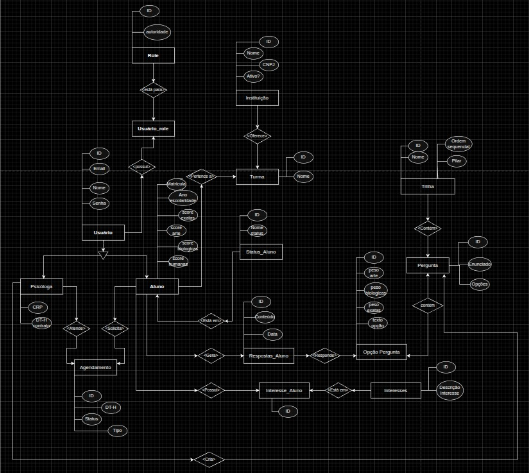
\includegraphics[width=0.90\textwidth]{img/diag-2-modelo-entidade-relacionamento.png}
    \legend{Fonte: Autoria própria (2026).}
\end{figure}

\subsection{Diagrama Entidade Relacionamento -- DER (Tabelas)}

O diagrama abaixo representa a estrutura física do banco de dados, detalhando as tabelas e suas respectivas chaves primárias e estrangeiras:

\begin{figure}[H]
    \centering
    \caption{Diagrama Entidade Relacionamento (DER) do SyncCarreira.}
    \label{fig_der}
    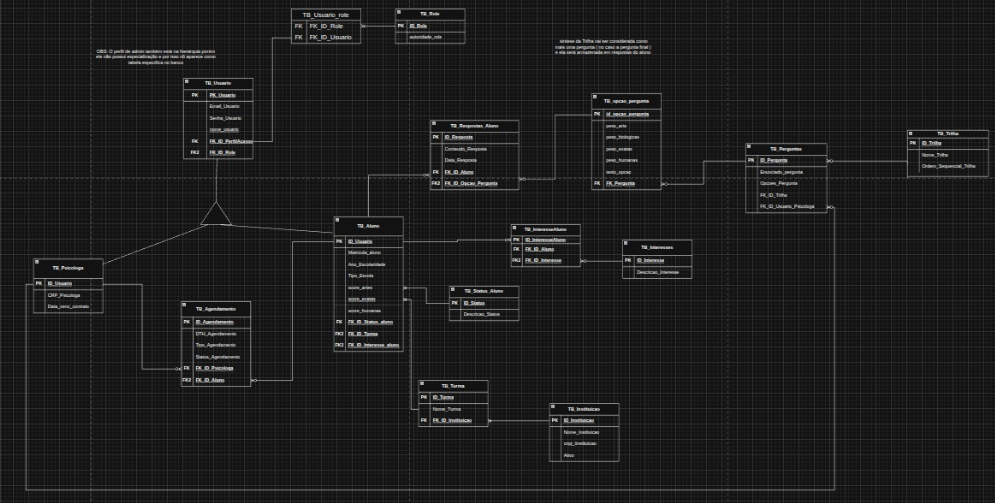
\includegraphics[width=0.90\textwidth]{img/diag-3-diagrama-entidade-relacionamento.png}
    \legend{Fonte: Autoria própria (2026).}
\end{figure}

\subsection{Dicionário de Dados}

O dicionário de dados tem como objetivo documentar de forma detalhada os elementos armazenados no banco de dados do sistema \textit{SyncCarreira}, descrevendo suas tabelas, atributos, tipos de dados, restrições e finalidades. Essa documentação auxilia na manutenção, evolução e compreensão da estrutura de dados utilizada pela aplicação. A modelagem segue os princípios da Terceira Forma Normal (3FN), garantindo integridade e reduzindo redundâncias.

\begin{table}[htb]
\ABNTEXfontereduzida
\caption[Dicionário de Dados do SyncCarreira]{Dicionário de dados do SyncCarreira.}
\label{tab-dicionario}
\begin{tabular}{p{2.5cm}|p{4cm}|p{7.5cm}}
\textbf{Tabela} & \textbf{Campo} & \textbf{Descrição} \\
\hline
Instituicao & id, nome, cnpj & Dados da escola ou ONG parceira. \\
\hline
Usuario & id, nome, perfil, senha & Cadastro de administradores, psicólogos e alunos. \\
\hline
Trilha & id, titulo, pilar, ordem & Configuração dos pilares da jornada (ex: Autoconhecimento). \\
\hline
Pergunta & id, texto, tipo & Questões associadas às trilhas de orientação. \\
\hline
Resposta & id, valor, síntese & Registros das interações e reflexões do aluno. \\
\hline
Agendamento & id, data, status & Registros de sessões e orientações da psicóloga. \\
\end{tabular}
\legend{Fonte: Autoria própria (2026).}
\end{table}

% --- TABELA: INSTITUIÇÃO ---
\begin{table}[H]
    \centering
    \ABNTEXfontereduzida
    \caption[Dicionário de Dados - Tabela Instituição]{Dicionário de dados: Tabela Instituição.}
    \label{tab-tb-instituicao}
    \begin{tabular}{p{3.5cm}|p{2cm}|c|p{3.5cm}|p{4cm}}
    \textbf{Campo} & \textbf{Tipo} & \textbf{Tamanho} & \textbf{Restrição} & \textbf{Descrição} \\
    \hline
    ID\_Instituicao & INT & - & PK, AUTO\_INCREMENT & Identificador único da instituição \\
    \hline
    Nome\_Instituicao & VARCHAR & 150 & NOT NULL & Nome da instituição \\
    \hline
    CNPJ\_Instituicao & CHAR & 14 & UNIQUE, NOT NULL & CNPJ da instituição \\
    \hline
    Ativo & BOOLEAN & - & NOT NULL & Indica se a instituição está ativa \\
    \end{tabular}
    \legend{Fonte: Autoria própria (2026).}
\end{table}

% --- TABELA: USUÁRIO ---
\begin{table}[H]
    \centering
    \ABNTEXfontereduzida
    \caption[Dicionário de Dados - Tabela Usuário]{Dicionário de dados: Tabela Usuário.}
    \label{tab-tb-usuario}
    \begin{tabular}{p{3.5cm}|p{2cm}|c|p{3.5cm}|p{4cm}}
    \textbf{Campo} & \textbf{Tipo} & \textbf{Tamanho} & \textbf{Restrição} & \textbf{Descrição} \\
    \hline
    ID\_Usuario & INT & - & PK, AUTO\_INCREMENT & Identificador único do usuário \\
    \hline
    Nome\_Usuario & VARCHAR & - & NOT NULL & Nome completo do Usuário \\
    \hline
    Email\_Usuario & VARCHAR & 150 & UNIQUE, NOT NULL & E-mail utilizado para autenticação no sistema \\
    \hline
    Senha\_Usuario & VARCHAR & 255 & NOT NULL & Senha criptografada do usuário \\
    \hline
    FK\_ID\_PerfilAcesso & INT & - & FK, NOT NULL & Referência ao perfil de acesso do usuário \\
    \end{tabular}
    \legend{Fonte: Autoria própria (2026).}
\end{table}

    Observação: Na modelagem, Aluno é uma especialização de Usuário, utilizando o mesmo identificador.

% --- TABELA: AGENDAMENTO ---
\begin{table}[H]
    \centering
    \ABNTEXfontereduzida
    \caption[Dicionário de Dados - Tabela Agendamento]{Dicionário de dados: Tabela Agendamento.}
    \label{tab-tb-agendamento}
    \begin{tabular}{p{3.5cm}|p{2cm}|c|p{3.5cm}|p{4cm}}
    \textbf{Campo} & \textbf{Tipo} & \textbf{Tamanho} & \textbf{Restrição} & \textbf{Descrição} \\
    \hline
    ID\_Agendamento & INT & - & PK, AUTO\_INCREMENT & Identificador único do agendamento \\
    \hline
    DTH\_Agendamento & DATETIME & - & NOT NULL & Data e hora do atendimento \\
    \hline
    Tipo\_Agendamento & VARCHAR & 50 & NOT NULL & Tipo do atendimento agendado \\
    \hline
    Status\_Agendamento & VARCHAR & 30 & NOT NULL & Situação atual do agendamento \\
    \hline
    FK\_ID\_Psicologa & INT & - & FK, NOT NULL & Psicóloga responsável \\
    \hline
    FK\_ID\_Aluno & INT & - & FK, NOT NULL & Aluno atendido \\
    \end{tabular}
    \legend{Fonte: Autoria própria (2026).}
\end{table}

% --- TABELA: PERGUNTA ---
\begin{table}[H]
    \centering
    \ABNTEXfontereduzida
    \caption[Dicionário de Dados - Tabela Pergunta]{Dicionário de dados: Tabela Pergunta.}
    \label{tab-tb-pergunta}
    \begin{tabular}{p{3.5cm}|p{2cm}|c|p{3.5cm}|p{4cm}}
    \textbf{Campo} & \textbf{Tipo} & \textbf{Tamanho} & \textbf{Restrição} & \textbf{Descrição} \\
    \hline
    ID\_Pergunta & INT & - & PK, AUTO\_INCREMENT & Identificador único da pergunta \\
    \hline
    Enunciado\_Pergunta & TEXT & - & NOT NULL & Texto da pergunta apresentada ao aluno \\
    \hline
    Opcoes\_Pergunta & TEXT & - & NOT NULL & Conjunto de alternativas disponíveis \\
    \hline
    FK\_ID\_Usuario & INT & - & FK & ID da psicóloga \\
    \hline
    FK\_ID\_Trilha & INT & - & FK, NOT NULL & ID externo da trilha \\
    \end{tabular}
    \legend{Fonte: Autoria própria (2026).}
\end{table}

Observação: A síntese da trilha será tratada como uma questão discursiva adicional, posicionada ao término do questionário. Seu objetivo é possibilitar que o aluno expresse, de forma livre, suas reflexões, percepções e interpretações acerca das experiências e conteúdos trabalhados durante a trilha. A inclusão dessa etapa amplia a capacidade analítica do sistema ao incorporar dados qualitativos, contribuindo para uma avaliação mais abrangente, personalizada e aderente às particularidades de cada estudante.

% --- TABELA: TRILHA ---
\begin{table}[H]
    \centering
    \ABNTEXfontereduzida
    \caption[Dicionário de Dados - Tabela Trilha]{Dicionário de dados: Tabela Trilha.}
    \label{tab-tb-trilha}
    \begin{tabular}{p{3.5cm}|p{2cm}|c|p{3.5cm}|p{4cm}}
    \textbf{Campo} & \textbf{Tipo} & \textbf{Tamanho} & \textbf{Restrição} & \textbf{Descrição} \\
    \hline
    ID\_Trilha & INT & - & PK, AUTO\_INCREMENT & Identificador único da trilha \\
    \hline
    Nome\_Trilha & VARCHAR & 100 & NOT NULL & Nome da trilha \\
    \hline
    Ordem\_Sequencial\_Trilha & INT & - & NOT NULL & Ordem de exibição da trilha \\
    \hline
    Pilar & VARCHAR & 100 & NOT NULL & Pilar de desenvolvimento relacionado \\
    \hline
    FK\_ID\_Perguntas & INT & - & FK, NOT NULL & Pergunta associada à trilha \\
    \end{tabular}
    \legend{Fonte: Autoria própria (2026).}
\end{table}

% --- TABELA: RESPOSTA ---
\begin{table}[H]
    \centering
    \ABNTEXfontereduzida
    \caption[Dicionário de Dados - Tabela Resposta]{Dicionário de dados: Tabela Resposta.}
    \label{tab-tb-resposta}
    \begin{tabular}{p{3.5cm}|p{2cm}|c|p{3.5cm}|p{4cm}}
    \textbf{Campo} & \textbf{Tipo} & \textbf{Tamanho} & \textbf{Restrição} & \textbf{Descrição} \\
    \hline
    ID\_Resposta & INT & - & PK, AUTO\_INCREMENT & Identificador único da resposta \\
    \hline
    Conteudo\_Resposta & TEXT & - & NOT NULL & Resposta fornecida pelo aluno \\
    \hline
    Data\_Resposta & DATETIME & - & NOT NULL & Data e hora da resposta \\
    \hline
    FK\_ID\_Aluno & INT & - & FK, NOT NULL & Aluno que respondeu \\
    \end{tabular}
    \legend{Fonte: Autoria própria (2026).}
\end{table}

% --- TABELA: INTERESSE ---
\begin{table}[H]
    \centering
    \ABNTEXfontereduzida
    \caption[Dicionário de Dados - Tabela Interesse]{Dicionário de dados: Tabela Interesse.}
    \label{tab-tb-interesse}
    \begin{tabular}{p{3.5cm}|p{2cm}|c|p{3.5cm}|p{4cm}}
    \textbf{Campo} & \textbf{Tipo} & \textbf{Tamanho} & \textbf{Restrição} & \textbf{Descrição} \\
    \hline
    ID\_Interesse & INT & - & PK, AUTO\_INCREMENT & Identificador único do interesse \\
    \hline
    Descricao\_Interesse & VARCHAR & 150 & NOT NULL & Descrição do interesse profissional \\
    \end{tabular}
    \legend{Fonte: Autoria própria (2026).}
\end{table}

% --- TABELA: INTERESSE ALUNO ---
\begin{table}[H]
    \centering
    \ABNTEXfontereduzida
    \caption[Dicionário de Dados - Tabela Interesse Aluno]{Dicionário de dados: Tabela Interesse Aluno.}
    \label{tab-tb-interesse-aluno}
    \begin{tabular}{p{3.5cm}|p{2cm}|c|p{3.5cm}|p{4cm}}
    \textbf{Campo} & \textbf{Tipo} & \textbf{Tamanho} & \textbf{Restrição} & \textbf{Descrição} \\
    \hline
    ID\_InteresseAluno & INT & - & PK, AUTO\_INCREMENT & Identificador único do relacionamento \\
    \hline
    FK\_ID\_Aluno & INT & - & FK, NOT NULL & Aluno associado \\
    \hline
    FK\_ID\_Interesse & INT & - & FK, NOT NULL & Interesse associado \\
    \end{tabular}
    \legend{Fonte: Autoria própria (2026).}
\end{table}

% --- TABELA: ROLE ---
\begin{table}[H]
    \centering
    \ABNTEXfontereduzida
    \caption[Dicionário de Dados - Tabela Role]{Dicionário de dados: Tabela Role.}
    \label{tab-tb-role}
    \begin{tabular}{p{3.5cm}|p{2cm}|c|p{3.5cm}|p{4cm}}
    \textbf{Campo} & \textbf{Tipo} & \textbf{Tamanho} & \textbf{Restrição} & \textbf{Descrição} \\
    \hline
    ID\_Role & INT & - & PK, AUTO\_INCREMENT & Identificador único da role \\
    \hline
    Autoridade\_Role & VARCHAR & 100 & NOT NULL & Nome da autoridade/permissão \\
    \end{tabular}
    \legend{Fonte: Autoria própria (2026).}
\end{table}

% --- TABELA: USUARIO ROLE ---
\begin{table}[H]
    \centering
    \ABNTEXfontereduzida
    \caption[Dicionário de Dados - Tabela Usuario Role]{Dicionário de dados: Tabela Usuario Role.}
    \label{tab-tb-usuario-role}
    \begin{tabular}{p{3.5cm}|p{2cm}|c|p{3.5cm}|p{4cm}}
    \textbf{Campo} & \textbf{Tipo} & \textbf{Tamanho} & \textbf{Restrição} & \textbf{Descrição} \\
    \hline
    FK\_ID\_Usuario & INT & - & PK, FK, NOT NULL & Usuário associado \\
    \hline
    FK\_ID\_Role & INT & - & PK, FK, NOT NULL & Role associada \\
    \end{tabular}
    \legend{Fonte: Autoria própria (2026).}
\end{table}

% --- TABELA: PSICÓLOGA ---
\begin{table}[H]
    \centering
    \ABNTEXfontereduzida
    \caption[Dicionário de Dados - Tabela Psicóloga]{Dicionário de dados: Tabela Psicóloga.}
    \label{tab-tb-psicologa}
    \begin{tabular}{p{3.5cm}|p{2cm}|c|p{3.5cm}|p{4cm}}
    \textbf{Campo} & \textbf{Tipo} & \textbf{Tamanho} & \textbf{Restrição} & \textbf{Descrição} \\
    \hline
    ID\_Usuario & INT & - & PK, FK & Referência ao usuário \\
    \hline
    CRP\_Psicologa & VARCHAR & 20 & UNIQUE, NOT NULL & Registo profissional da psicóloga \\
    \hline
    Dias\_Ver\_Cronograma & BOOLEAN & - & NOT NULL & Define se pode visualizar cronogramas \\
    \end{tabular}
    \legend{Fonte: Autoria própria (2026).}
\end{table}

Observação: Na modelagem, Psicóloga é uma especialização de Usuário, utilizando o mesmo identificador.

% --- TABELA: OPÇÃO PERGUNTA ---
\begin{table}[H]
    \centering
    \ABNTEXfontereduzida
    \caption[Dicionário de Dados - Tabela Opção Pergunta]{Dicionário de dados: Tabela Opção Pergunta.}
    \label{tab-tb-opcao-pergunta}
    \begin{tabular}{p{3.5cm}|p{2cm}|c|p{3.5cm}|p{4cm}}
    \textbf{Campo} & \textbf{Tipo} & \textbf{Tamanho} & \textbf{Restrição} & \textbf{Descrição} \\
    \hline
    ID\_Opcao\_Pergunta & INT & - & PK, AUTO\_INCREMENT & Identificador único da opção \\
    \hline
    Peso\_Alta & INT & - & NOT NULL & Pontuação atribuída ao pilar Alta \\
    \hline
    Peso\_Biologica & INT & - & NOT NULL & Pontuação atribuída ao pilar Biológica \\
    \hline
    Peso\_Interesse & INT & - & NOT NULL & Pontuação atribuída ao pilar Interesse \\
    \hline
    Peso\_Social & INT & - & NOT NULL & Pontuação atribuída ao pilar Social \\
    \hline
    FK\_ID\_Pergunta & INT & - & FK, NOT NULL & Pergunta à qual a opção pertence \\
    \end{tabular}
    \legend{Fonte: Autoria própria (2026).}
\end{table}
\section{Duração / Cronograma}

O projeto \textit{SyncCarreira} possui uma estimativa total de execução de 10 meses, divididos em duas fases principais. A primeira fase foca no planejamento e na entrega de um Produto Mínimo Viável (MVP), enquanto a segunda fase foca na escala, integração de recursos avançados e testes de carga.

\subsection{Análise da Duração do Projeto}

Abaixo, apresentamos o cronograma detalhado por semanas de desenvolvimento:

\begin{table}[htb]
\ABNTEXfontereduzida
\caption[Cronograma de Desenvolvimento do SyncCarreira]{Cronograma de desenvolvimento do SyncCarreira.}
\label{tab-cronograma}
\begin{tabular}{p{2.5cm}|p{4.5cm}|p{2cm}|p{5cm}}
\textbf{Fase} & \textbf{Atividade} & \textbf{Duração} & \textbf{Entregável principal} \\
\hline
I. Concepção & Levantamento de Requisitos e Análise de Mercado & 3 semanas & Documento de Visão e RF/RNF \\
\hline
I. Concepção & Modelagem de Dados e Arquitetura UML & 2 semanas & DER, Diagramas de Classes e Componentes \\
\hline
II. MVP & Configuração do Ambiente (Java/Spring/DB) & 1 semana & Repositório e Pipeline CI/CD \\
\hline
II. MVP & Desenvolvimento do Módulo de Autenticação (OAuth2/JWT) & 2 semanas & Sistema de Login funcional \\
\hline
II. MVP & Motor de Testes e Persistência de Respostas & 4 semanas & Fluxo principal do teste vocacional \\
\hline
II. MVP & Painel Básico (\textit{Frontend} SPA) & 3 semanas & Interface de acompanhamento inicial \\
\hline
II. MVP & Testes Unitários e Integração (Core) & 2 semanas & Relatório de cobertura de testes \\
\hline
III. Refino & Curadoria e Trilhas de Informação & 4 semanas & Banco de dados de artigos e trilhas \\
\hline
III. Refino & Módulo de Feedbacks e Agendamentos & 3 semanas & Funcionalidade de interação Psicóloga-Aluno \\
\hline
IV. Escala & Dashboard de Análise e Relatórios (PDF/BI) & 5 semanas & Gerador de relatórios e Dashboards \\
\hline
IV. Escala & Testes de Performance, Carga e Segurança & 3 semanas & Relatório de estabilidade e segurança \\
\hline
V. Encerramento & Deploy Final e Homologação & 2 semanas & Sistema em ambiente de produção \\
\end{tabular}
\legend{Fonte: Autoria própria (2026).}
\end{table}
